Let $f$ be defined by $f(t)=0$ for $t<0$; $f(t)=t$ for $0\leq t\leq1$; $f(t)=4$ for $t>1$.\\

a. Determine the function $F(x)=\int_0^xf(t)dt$.\\

b. Sketch. Where is $F$ continuous?\\

c. Where is $F$ differentiable and find $F'$ at those values.\\\\

\begin{solution}\renewcommand{\qedsymbol}{}\ \\
    Well, $F(x)=0$ for $x<0$; $F(x)=x^2$ for $0\leq x\leq1$; and $F(x)=4x$ for $x>1$.\\

    \begin{center}
        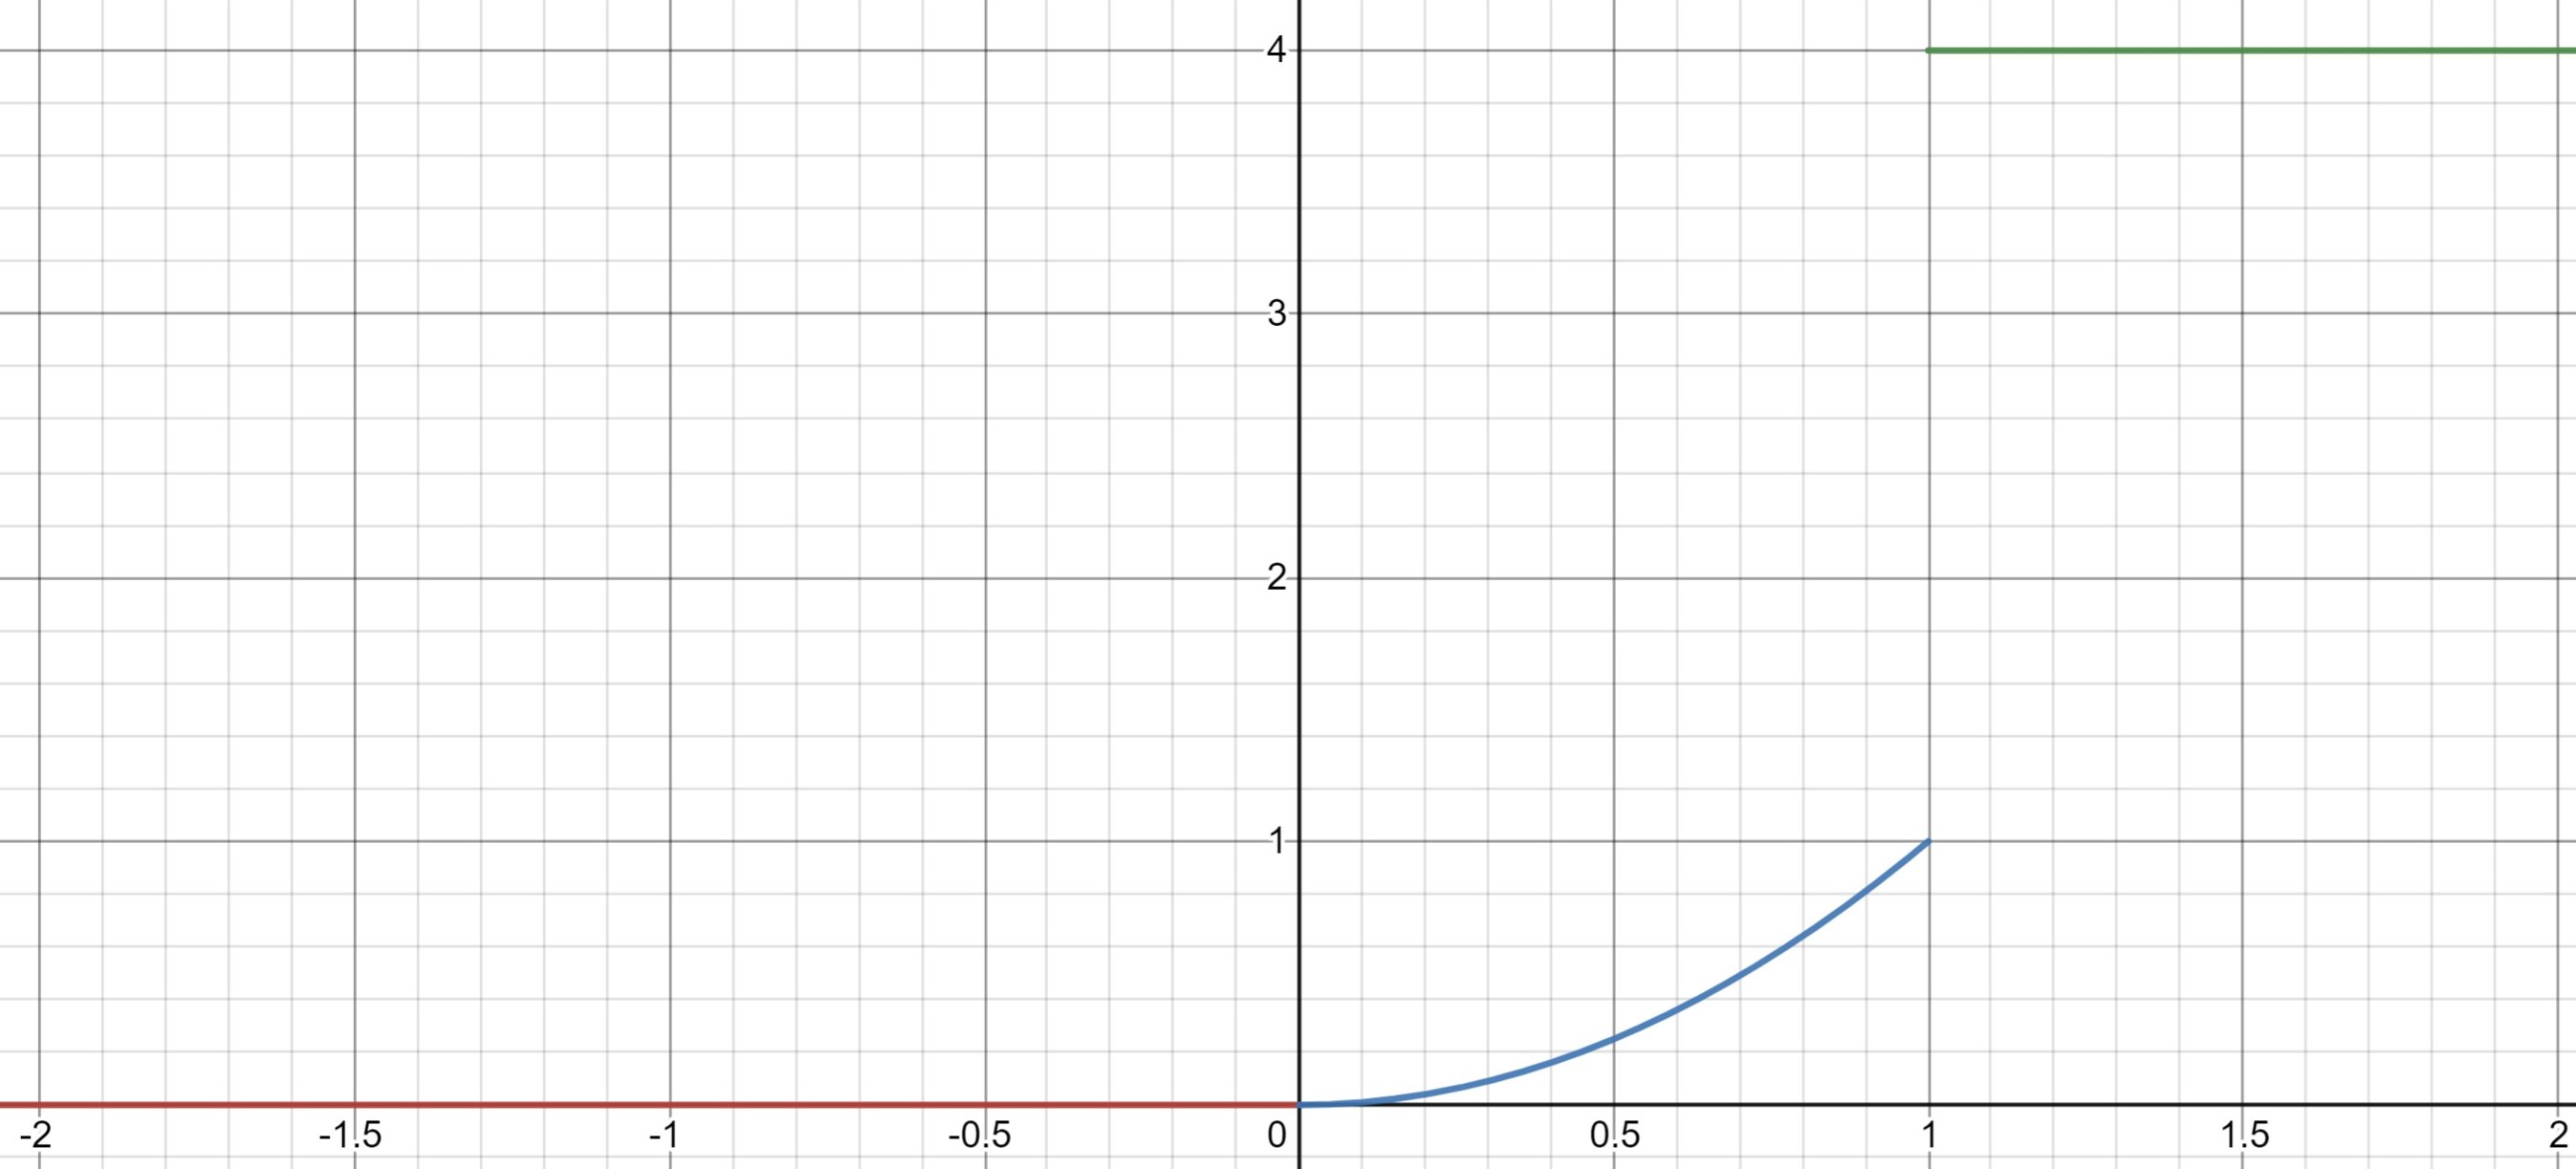
\includegraphics[scale=0.5]{graph F.JPG}\\
    \end{center}

    $F$ is continuous on $\{x|x\neq1\}$\\

    $F$ is differentiable on $\{x|x\neq1\}$ and $F'=0$ for $x<0$, $F'=t$ for $0\leq x<1$, and $F'=4$ for
    $x>1$.

\end{solution}